\chapter{Revisão da literatura}

\section{Redes complexas e grafos}

Estamos rodeados por sistemas irremediavelmente complexos que envolvem interações em grande escala. Exemplos disso incluem sociedades com bilhões de indivíduos cooperando, infraestruturas de comunicação conectando milhões de telemóveis, computadores e satélites, e a atividade coordenada de bilhões de neurônios em nosso cérebro para compreender o mundo. Além disso, nossa biologia depende de inúmeras interações entre genes e metabolitos nas células \cite{Albert_2002}.

Esses sistemas são chamados coletivamente de sistemas complexos devido à dificuldade em prever seu comportamento com base no conhecimento de seus componentes individuais. Dada a importância desses sistemas em nossa vida cotidiana, na ciência e na economia, compreender, descrever matematicamente, prever e até controlar sistemas complexos se tornou um dos principais desafios intelectuais e científicos do século XXI.

Um recurso fundamental para abordar essa complexidade é a teoria dos grafos, que representa sistemas como conjuntos de nós interconectados por arestas. As redes são uma poderosa abordagem para estudar sistemas complexos em diversas áreas, como biologia, sociologia, tecnologia e transporte \cite{barabasi2016network}.

\begin{figure}[!h]
    \centering
    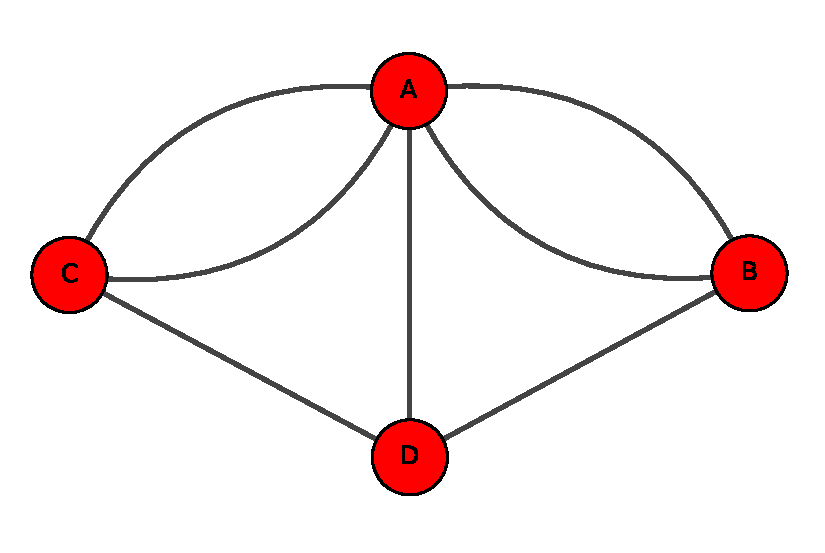
\includegraphics[width=8cm]{figures/konigsberg.pdf}
    \caption{A figura apresenta o grafo que descreve a solução do famoso problema das sete pontes de Königsberg. Este desafio histórico, resolvido por \citeonline{Euler1736}, originou a teoria dos grafos.}
    \label{fig:basin-region}
\end{figure}

Os links de uma rede podem ser direcionados ou não direcionados, e essa distinção desempenha um papel crucial na modelagem de sistemas complexos. Redes com links direcionados, como a World Wide Web (WWW) ou chamadas telefônicas, têm conexões unilaterais, onde a direção importa, indicando que um nó está conectado a outro de forma diferente da recíproca. Por outro lado, redes não direcionadas, como relacionamentos ou linhas de transmissão elétrica, refletem conexões bidirecionais, onde a relação é simétrica. Além disso, algumas redes combinam ambos os tipos de conexões, como as redes metabólicas, onde algumas reações são reversíveis (bidirecionais) e outras são irreversíveis (direcionadas).

A representação matemática de uma rede é essencial para sua análise. Uma rede é formalmente definida como um grafo $G(V, E)$, onde $V$ representa os nós (ou vértices) da rede e $E$ representa as arestas (ou links) entre esses nós. Dentro deste contexto, muitas vezes trabalhamos com redes ponderadas, onde os pesos das arestas ($W_{ij}$) entre pares de nós ($i$ e $j$) representam valores como fluxos, distâncias ou outras medidas relevantes para o sistema. Essa abordagem matemática permite a aplicação de técnicas de análise de grafos para entender a topologia e dinâmica das redes complexas que permeiam nosso mundo \cite{Newman2010}.

Uma descrição completa de uma rede exige que acompanhemos seus links. A maneira mais simples de conseguir isso é fornecer uma lista completa dos links \cite{barabasi2016network}. Para fins matemáticos, frequentemente representamos uma rede através de sua matriz de adjacência. A matriz de adjacência de uma rede direcionada de $N$ nós possui $N$ linhas e $N$ colunas, sendo seus elementos:
\begin{align*}
    A_{ij} =
    \begin{cases}
        1, & \text{se existe um link apontando do nó } j \text{ para o nó } i \\
        0, & \text{se os nós } i \text{ e } j \text{ não estiverem conectados entre si}
    \end{cases}
\end{align*}

A matriz de adjacência de uma rede não direcionada possui duas entradas para cada link, por ex. o link (1, 2) é representado como $A_{12} = 1$ e $A_{21} = 1$. Portanto, a matriz de adjacência de uma rede não direcionada é simétrica, $A_{ij} = A_{ji}$.

A matriz de adjacência desempenha um papel fundamental na análise de redes, pois permite representar de forma clara e concisa a conectividade entre os nós. Ela é especialmente útil para calcular propriedades como o grau dos nós, identificar subgrafos e realizar diversas análises matemáticas e estatísticas sobre a rede. Além disso, a matriz de adjacência pode ser empregada em algoritmos que exploram a estrutura da rede para resolver uma variedade de problemas, desde encontrar caminhos mais curtos até identificar comunidades de nós.

Portanto, a matriz de adjacência desempenha um papel central na análise e modelagem de redes complexas, permitindo-nos explorar e compreender as interações entre seus componentes.

\section{Redes temporais}

A compreensão de sistemas complexos, sejam eles biológicos, sociais ou tecnológicos, muitas vezes exige uma perspectiva de longo alcance que nos permita observar a organização global e suas interações fundamentais. A modelagem de redes oferece uma abordagem valiosa para simplificar a complexidade, concentrando-se nas unidades e conexões que compõem esses sistemas. No entanto, uma dimensão crucial muitas vezes negligenciada é o tempo. 

A rede temporal, uma extensão da modelagem de redes, aborda essa lacuna ao não apenas considerar quais unidades estão interconectadas, mas também quando essas interações ocorrem. Essa abordagem não se limita apenas a sistemas biológicos ou sociais, mas abrange uma ampla gama de contextos, desde infraestruturas tecnológicas até interações ecológicas. Ao incorporar o fator temporal, as redes temporais nos capacitam a capturar nuances e dinâmicas que podem ser essenciais para uma compreensão completa dos sistemas em estudo \cite{HOLME201297}.

As redes dinâmicas, aquelas que evoluem ao longo do tempo, desempenham um papel de destaque na compreensão dos processos de disseminação, abrangendo desde a propagação de informações até a disseminação de doenças \cite{HOLME201297}. Isso se deve ao fato de que, em tais redes, cada conexão entre elementos representa uma oportunidade de interação, e a sequência temporal dessas interações é cuidadosamente registrada.

As escalas de tempo, representadas por $t_N$ e $t_P$, desempenham um papel fundamental na análise de redes temporais. O valor de $t_N$ refere-se à escala de tempo característica para a evolução da própria rede, ou seja, quanto tempo leva para que a estrutura da rede se modifique de maneira significativa. Por outro lado, $t_P$ representa a escala de tempo característica para a dinâmica do processo de propagação que ocorre sobre essa rede.

Em cenários onde $t_N$ é consideravelmente maior do que $t_P$ (ou seja, $t_N \gg t_P$), a rede evolui em um ritmo relativamente lento em comparação com a dinâmica do processo, tornando possível uma abordagem estática da rede para simplificar a modelagem do fenômeno em questão. No entanto, quando $t_N$ e $t_P$ são da mesma ordem de grandeza (ou seja, $t_N \sim t_P$), as redes temporais se destacam, pois a interação entre a evolução da rede e o processo de propagação torna-se significativa e não pode ser negligenciada. Por fim, em cenários onde a rede evolui rapidamente em relação ao processo (ou seja, $t_N \ll t_P$), pode ser apropriado usar uma abordagem de rede média no tempo para simplificar a modelagem.

Essa distinção entre as escalas de tempo nos permite escolher a abordagem mais adequada para cada situação, adaptando-a à natureza e à temporalidade dos processos em sistemas complexos.

\section{Modelos epidemiológicos}

A modelagem em epidemiologia compartilha objetivos similares com a modelagem ecológica, centrando-se na compreensão da prevalência, distribuição e fatores que influenciam a incidência, propagação e persistência de doenças. Enquanto na ecologia, a quantificação precisa da abundância de espécies frequentemente é de grande interesse, na epidemiologia, o foco recai na categorização dos indivíduos de acordo com seu estado de infecção em uma população hospedeira \cite{Matt2008}. Nesse contexto, os modelos epidemiológicos podem ser comparados aos modelos de metapopulação da ecologia \cite{macarthur1967theory, levins1969demographic}, onde cada indivíduo é considerado como um recurso para o patógeno, com processos de transmissão e recuperação análogos à dispersão e extinção. A modelagem matemática em epidemiologia tem uma longa história e tem sido aplicada desde o século XVIII, passando por desenvolvimentos conceituais e técnicos significativos.

A modelagem de epidemias envolve duas abordagens principais: estocástica e determinística.

Nos modelos estocásticos, a aleatoriedade está presente nas variáveis, permitindo estimar distribuições de probabilidade de resultados possíveis, especialmente quando as flutuações aleatórias têm um papel significativo, como em populações pequenas ou em cenários com variações casuais marcantes.

Por outro lado, os modelos determinísticos são empregados para grandes populações, como por exemplo para o estudo da tuberculose. Neles, a população é dividida em compartimentos representando diferentes estágios da epidemia. As taxas de transição entre esses compartimentos são descritas por equações diferenciais.

Além disso, é importante destacar que, ao longo deste estudo, trabalharemos com a suposição de que a população em análise apresenta uma mistura homogênea, ou seja, todos os indivíduos interagem igualmente entre si \cite{allman_rhodes_2003}. Essa premissa implica que o risco de exposição à doença por parte dos não infectados é uniforme em relação aos indivíduos já infectados.

\subsection{Modelo SIR}

O modelo epidêmico mais simples, porém poderoso, que podemos considerar é o modelo SIR. Neste, os membros da população progridem através de três compartimentos, da seguinte forma:
\begin{itemize}
    \item \textcolor{hexagram}{\textbf{Suscetíveis (S)}}: Esta classe representa os indivíduos que estão em risco de contrair a doença, mas que atualmente não estão infectados.
    \item \textcolor{hexagram1}{\textbf{Infectados (I)}}: Aqui, encontramos aqueles que já foram infectados pela doença e são atualmente contagiosos.
    \item \textcolor{hexagram2}{\textbf{Removidos (R)}}: Esta classe abrange os indivíduos que não podem mais contrair a doença, seja porque se recuperaram completamente, desenvolveram imunidade natural ou, infelizmente, faleceram.
\end{itemize}

\begin{figure}[!h]
    \centering
    
\includegraphics[width=8cm]{figures/SIRmodel.png}
    \caption{Diagrama esquemático do modelo SIR, adaptado de \citeonline{barabasi2016network}.}
    \label{fig:SIR}
\end{figure}

A evolução de uma epidemia, como a da gripe, muitas vezes ocorre em um ritmo muito mais acelerado em comparação com as mudanças na taxa de natalidade e mortalidade. Como resultado, modelos compartimentais simplificados frequentemente excluem considerações sobre nascimentos e mortes, um aspecto conhecido como dinâmica vital (ou demografia). O sistema SIR sem a influência da dinâmica vital, para uma população com $N$ hospedeiros, pode ser representado por meio do seguinte conjunto de equações diferenciais ordinárias \cite{Hethcote2000}:
{\large
\begin{align}
\label{eq:sistema_equacoes}
\begin{cases}
\frac{dS}{dt} = -\frac{{\boldsymbol{\beta}} S I}{N}, \\
\frac{dI}{dt} = \frac{{\boldsymbol{\beta}} S I}{N} - \gamma I, \\
\frac{dR}{dt} = \gamma I.
\end{cases}
\end{align}}

Apesar de sua não linearidade, este sistema possibilita uma solução analítica implícita \cite{Harko2014}. Inicialmente, observe a seguinte relação:

{\large
\begin{equation}\label{eq:conservacao_populacao}
\frac{dS}{dt} + \frac{dI}{dt} + \frac{dR}{dt} = 0
\end{equation}}
Pode-se deduzir que:
{\large
\begin{equation}\label{eq:conservacao_populacao2}
S(t) + I(t) + R(t) = \text{constante} = N
\end{equation}}
A invariabilidade da população $N$ simplifica a análise, permitindo a consideração de apenas duas das três variáveis em questão.

A taxa de transmissão, $\beta$, é uma medida da probabilidade de um indivíduo infectado transmitir a doença a um indivíduo suscetível. Por exemplo, se $\beta$ for $0.1$, então um indivíduo infectado tem $10$\% de probabilidade de transmitir a doença a um indivíduo suscetível, ao entrar em contato com o mesmo, em um determinado período de tempo.

A taxa de recuperação, $\gamma$, é uma medida da rapidez com que um indivíduo infectado se recupera da doença. Por exemplo, se $\gamma$ for $0.2$, então um indivíduo infectado se recuperará da doença dentro de $5$ dias.

As unidades $\beta$ e $\gamma$ são importantes porque determinam o comportamento do modelo SIR. Se $\beta$ for maior que $\gamma$, então a doença se espalhará pela população. Se $\beta$ for menor que $\gamma$, a doença desaparecerá.

Em conjunto, esses dois parâmetros do modelo nos fornecem o \textit{número básico de  reprodução} $R_{0}$: uma medida representativa do número médio de infecções secundárias originadas a partir de um hospedeiro já infectado.

{\large
\begin{equation}
R_0 = \frac{\beta}{\gamma}
\label{eq:R0}
\end{equation}}

No cenário onde o valor de $R_{0}$ ultrapassa a marca de um, a taxa de infecção supera a taxa de recuperação, o que resulta no crescimento da infecção em toda a população. Por outro lado, quando $R_{0}$ permanece abaixo de um, a infecção tende a desaparecer rapidamente, uma vez que as pessoas se recuperam mais rapidamente do que contribuem para a propagação da doença.